%%%%%%%%%%%%  Generated using docx2latex.com  %%%%%%%%%%%%%%

%%%%%%%%%%%%  v2.0.0-beta  %%%%%%%%%%%%%%

\documentclass[12pt]{article}
\usepackage{amsmath}
\usepackage{latexsym}
\usepackage{amsfonts}
\usepackage[normalem]{ulem}
\usepackage{soul}
\usepackage{array}
\usepackage{amssymb}
\usepackage{extarrows}
\usepackage{graphicx}
\usepackage[backend=biber,
style=numeric,
sorting=none,
isbn=false,
doi=false,
url=false,
]{biblatex}\addbibresource{bibliography.bib}

\usepackage{subfig}
\usepackage{wrapfig}
\usepackage{wasysym}
\usepackage{enumitem}
\usepackage{adjustbox}
\usepackage{ragged2e}
\usepackage[svgnames,table]{xcolor}
\usepackage{tikz}
\usepackage{longtable}
\usepackage{changepage}
\usepackage{setspace}
\usepackage{hhline}
\usepackage{multicol}
\usepackage{tabto}
\usepackage{float}
\usepackage{multirow}
\usepackage{makecell}
\usepackage{fancyhdr}
\usepackage[toc,page]{appendix}
\usepackage[hidelinks]{hyperref}
\usetikzlibrary{shapes.symbols,shapes.geometric,shadows,arrows.meta}
\tikzset{>={Latex[width=1.5mm,length=2mm]}}
\usepackage{flowchart}\usepackage[paperheight=11.0in,paperwidth=8.5in,left=0.79in,right=0.79in,top=0.79in,bottom=0.79in,headheight=1in]{geometry}
\usepackage[utf8]{inputenc}
\usepackage[T1]{fontenc}
\TabPositions{0.6in,1.2in,1.8in,2.4in,3.0in,3.6in,4.2in,4.8in,5.4in,6.0in,6.6in,}

\urlstyle{same}

\renewcommand{\_}{\kern-1.5pt\textunderscore\kern-1.5pt}

 %%%%%%%%%%%%  Set Depths for Sections  %%%%%%%%%%%%%%

% 1) Section
% 1.1) SubSection
% 1.1.1) SubSubSection
% 1.1.1.1) Paragraph
% 1.1.1.1.1) Subparagraph


\setcounter{tocdepth}{5}
\setcounter{secnumdepth}{5}


 %%%%%%%%%%%%  Set Depths for Nested Lists created by \begin{enumerate}  %%%%%%%%%%%%%%


\setlistdepth{9}
\renewlist{enumerate}{enumerate}{9}
		\setlist[enumerate,1]{label=\arabic*)}
		\setlist[enumerate,2]{label=\alph*)}
		\setlist[enumerate,3]{label=(\roman*)}
		\setlist[enumerate,4]{label=(\arabic*)}
		\setlist[enumerate,5]{label=(\Alph*)}
		\setlist[enumerate,6]{label=(\Roman*)}
		\setlist[enumerate,7]{label=\arabic*}
		\setlist[enumerate,8]{label=\alph*}
		\setlist[enumerate,9]{label=\roman*}

\renewlist{itemize}{itemize}{9}
		\setlist[itemize]{label=$\cdot$}
		\setlist[itemize,1]{label=\textbullet}
		\setlist[itemize,2]{label=$\circ$}
		\setlist[itemize,3]{label=$\ast$}
		\setlist[itemize,4]{label=$\dagger$}
		\setlist[itemize,5]{label=$\triangleright$}
		\setlist[itemize,6]{label=$\bigstar$}
		\setlist[itemize,7]{label=$\blacklozenge$}
		\setlist[itemize,8]{label=$\prime$}

\setlength{\topsep}{0pt}\setlength{\parindent}{0pt}
\renewcommand{\arraystretch}{1.3}


%%%%%%%%%%%%%%%%%%%% Document code starts here %%%%%%%%%%%%%%%%%%%%



\begin{document}
\setlength{\parskip}{21.6pt}
{\fontsize{14pt}{16.8pt}\selectfont \textbf{\textcolor[HTML]{00000A}{Coupling between tolerance and resistance differs between related \textit{Eimeria} parasite species: implications for coevolution with their mouse hosts}}\par}\par

\setlength{\parskip}{5.76pt}
{\fontsize{14pt}{16.8pt}\selectfont \textbf{Abstract}\par}\par

Resistance (host capacity to reduce parasite burden) and tolerance (host capacity to reduce impact on its health for a given parasite burden) manifest two different lines of defenses. Tolerance can be independent from resistance, traded-off against it, or the two can be positively correlated because of redundancy in underlying (immune) processes. We here tested whether closely related parasite species could show differences in this coupling between tolerance and resistance. \par

We tested this in infections with two parasite species of genus \textit{Eimeria. }We measured proxies for resistance (the (inverse of) number of parasite transmission stages (oocysts) per gram of feces at the day of maximal shedding) and tolerance (the slope of maximum relative weight loss compared to day of infection on number of oocysts per gram of feces at the day of maximal shedding for each host strain) in four inbred mouse strains belonging to two mouse subspecies, \textit{Mus musculus domesticus} and \textit{M. m. musculus}.\par

We found a negative correlation between resistance and tolerance against \textit{E. falciformis}, while the two are uncoupled against \textit{E. ferrisi.} We interpret this as indication that resistance and tolerance against the first parasite species might be traded off, but evolve independently in different mouse genotypes against the latter. We argue that host evolution can be studied largely irrespective of parasite strains if coupling is absent (\textit{E. ferrisi}) but host-parasite coevolution is more likely observable and best studied in a system with coupled tolerance and resistance (\textit{E. falciformis}). \par

\textbf{Keywords}: Resistance, Tolerance, Eimeria, Coevolution\par

{\fontsize{14pt}{16.8pt}\selectfont \textbf{Introduction}\par}\par

\setstretch{2.0}
\textcolor[HTML]{00000A}{H}ost defence mechanisms evolve to alleviate the detrimental effect of parasites. They can be categorised into two components: resistance and tolerance (Råberg, Graham, $\&$  Read, 2009). Resistance is the ability of a host to reduce parasite burden, resulting from defence against parasite infection or proliferation early after infection (Schmid-Hempel, 2013). The negative effect of resistance on parasite fitness can lead to antagonistic coevolution. According to theoretical models, fluctuating host and parasite genotypes arise, and balancing selection maintains resistance alleles polymorphic (Boots, Best, Miller, $\&$  White, 2008; Roy $\&$  Kirchner 2000)\textcolor[HTML]{666666}{.} Resistance has been the classical $``$catch all$"$  measure for host-parasite systems, but recently it has been shown to be incomplete, especially with respect to potential fitness effects on the host (Kutzer $\&$  Armitage, 2016; Råberg et al., 2009).\par

Disease tolerance (not to be confused from $``$immunological tolerance$"$ , unresponsiveness to self antigens; Medzhitov, Schneider, $\&$  Soares, 2012) is the ability of the host to limit the impact of parasite on its fitness (Råberg et al., 2009; Vale $\&$  Little, 2012; Kutzer $\&$  Armitage, 2016). By potentially providing a longer-living niche, this defence mechanism improves, or at least does not deteriorate, the fitness of the parasite. Tolerance alleles are thus predicted by theoretical models to evolve to fixation due to positive feedback loops (Boots et al., 2008; Restif $\&$  Koella, 2004; Roy $\&$  Kirchner 2000). From a mechanistic perspective tolerance alleviates direct or indirect (e.g. excessive immune response underlying resistance against parasites, called immunopathology; Graham, Allen, $\&$  Read, 2005) damage caused by parasites (Råberg et al., 2009). Tolerance mechanisms include modulation of inflammatory response (Ayres $\&$  Schneider, 2012), tissue repair (stress response, damage repair and cellular regeneration mechanisms; Soares, Teixeira, $\&$  Moita, 2017), and compensation of parasite‐induced damage by increase of reproductive effort (Baucom $\&$  de Roode, 2011). The resulting metabolic costs of resistance and tolerance, with and without parasites infection, determine the optimal (steady state and infection ineducable) extent and of both immune defences (Sheldon $\&$  Verhulst, 1996).\par

Resistance and tolerance can be genetically and physiologically independent, involving different proximate mechanisms. Lack of correlation between both defences was shown for example in monarch butterflies (\textit{Danaus plexippus}) infected by the protozoan parasite \textit{Ophryocystis elektroscirrha}. This study found genetic variation in resistance between butterflies families, but a fixed tolerance (Lefèvre, Williams, $\&$  de Roode, 2010). Similarly, no correlation could be found between resistance and tolerance for the fish \textit{Leuciscus burdigalensis} in response to infection with its parasite \textit{Tracheliastes polycolpus}. The authors explain the decoupling of both defences by the fact that, in this system, tolerance likely involves wound repair rather than immune regulation, making resistance and tolerance mechanisms independent (Mazé-Guilmo, Loot, Páez, Lefèvre, $\&$  Blanchet, 2014).\par

In other systems, the two lines of defense can rely on similar genes and mechanisms and be positively correlated. \textcolor[HTML]{FF0000}{For example, Guivier et al (2010) showed that \textit{Myodes glareolus} expresses the tumor necrosis factor-$ \alpha $  (TNF-$ \alpha $ ), a mediator of resistance to \textit{Puumala hantavirus }(PUUV) in several mammals, at a lower level in\textit{ }in PUUV endemic areas. These results suggest that the regulation of TNF-$ \alpha $  is both a resistance and a tolerance mechanism. Similarly, genetic association studies of resistance and tolerance of \textit{Drosophila melanogaster} against the bacterium \textit{Providencia rettgeri} have shown positively correlated genetic effects, as the same loci were associated with both traits (}Howick $\&$  Lazzaro, 2017). \par

Resistance and tolerance have been found negatively correlated in studies comparing distinct host populations or inbred host strains: Inbred laboratory mouse strains lose weight upon infection with \textit{Plasmodium chabaudi.} The extent of this impact on host health is negatively correlated with the peak number of parasites found in the blood (Råberg, Sim, $\&$  Read, 2007), meaning that mouse strains with higher resistance present lower tolerance. Similarly, infections of sea trout (Salmo trutta trutta) and Atlantic salmon (Salmo salar) with the trematode Diplostomum pseudospathaceum showed that resistance and tolerance were negatively correlated when assessing mean levels of both traits in different host populations (Klemme $\&$  Karvonen, 2016). This is interpreted as a result of trade-off between resistance and tolerance (Sheldon $\&$  Verhulst, 1996; Restif $\&$  Koella, 2004; Råberg et al., 2009).\par

\setlength{\parskip}{0.0pt}
We have seen that resistance and tolerance can be (1) uncoupled (independent), (2) positively correlated (involving same genes and mechanisms), or (3) negatively correlated (traded-off). Theoretical models show that coupling between resistance and tolerance (or absence thereof) depends not only on host factors, but is also conditioned by parasite intrinsic factors (Carval $\&$  Ferriere, 2010). Here, we tested differences in the resistance-tolerance coupling upon infection with two closely related parasite species. We infected four inbred mouse strains representative of two house mouse subspecies, \textit{M. m. domesticus} and \textit{M. m. musculus}, with three parasite isolates representative of two naturally occuring parasite species, the protozoan parasite \textit{Eimeria ferrisi} and \textit{E. falciformis }(Jarquín-Díaz et al. 2019). \textit{Eimeria }spp. are monoxenous parasites that expand asexually and reproduce sexually in intestinal epithelial cells, leading to malabsorption of nutrients, tissue damage and weight loss (Chapman et al., 2013). The evolutionary history of these different \textit{Eimeria} species in the two house mouse subspecies is unknown and it is unclear whether subspecies-specific adaptation exists in one or the other. We tested (1) if coupling between resistance and tolerance of each host differs between both parasite species; and (2) local adaptation of \textit{E. ferrisi} using a parasite isolated in a \textit{M. m. domesticus} host and one in a \textit{M. m. musculus} host.\par

\begin{FlushLeft}
{\fontsize{14pt}{16.8pt}\selectfont \textbf{Material and methods}\par}
\end{FlushLeft}\par

{\fontsize{14pt}{16.8pt}\selectfont \textbf{Parasite isolates}\par}\par

The three parasite isolates used in this study were isolated from feces of three different \textit{M. m. domesticus/M. m. musculus} hybrid mice captured in Brandenburg, Germany, in 2016 (capture permit No. 2347/35/2014). Hybrid index (HI) of each individual wild-caught mouse was calculated to account for the admixture of mouse genomes as a proportion of \textit{M. m. musculus} alleles in a set of 14 diagnostic markers (Balard et al., 2020). The parasite isolates belong to both the most prevalent \textit{Eimeria }species in this area, namely \textit{E. ferrisi }(isolates Brandenburg64 and Brandenburg139) and \textit{E. falciformis }(isolate Brandenburg88)(Jarquín-Díaz et al., 2019). Isolate Brandenburg64 was isolated in a 92$\%$  \textit{M. m. domesticus} individual (HI=0.08), isolate Brandenburg139 in a 85$\%$  \textit{M. m. musculus} (HI=0.85) and isolate Brandenburg88 in a 80$\%$  \textit{M. m. domesticus} (HI=0.2). Pre-patency and the peak day of parasite shedding for these isolates were estimated during infection in NMRI laboratory mice (Al-khlifeh et al., 2019) which were also used for serial passaging of all the isolates. Parasite infective forms (oocysts) were recovered by flotation in saturated NaCl solution followed by washing and observation under light microscope (following the protocol described in Clerc, Fenton, Babayan, $\&$  Pedersen, 2019) and stored at room temperature in 1mL of 2$\%$  potassium dichromate for a maximum of 2 months before infection of the wild-derived mouse strains. Oocysts were allowed to sporulate 10 days before infection in a water bath at 30$ ^{\circ} $ C.\par

\begin{FlushLeft}
{\fontsize{14pt}{16.8pt}\selectfont \textbf{Mouse strains}\par}
\end{FlushLeft}\par

We used four wild-derived inbred mouse strains \textcolor[HTML]{CE181E}{from which four F1 strains were bred. Two parental strains represented \textit{M. m. domesticus}: \textbf{SCHUNT} (Locality: Schweben, Hessen, Germany [N: 50$ ^{\circ} $  26’, E: 9$ ^{\circ} $  36’] (Martincov}á, Ďureje, Kreisinger, Macholán, $\&$  Piálek, 2019)) and \textbf{STRA} (Locality: Straas, Bavaria, Germany [N: 50$ ^{\circ} $  11’, E: 11$ ^{\circ} $  46’] (Piálek et al., 2008), and two derived from \textit{M. m. musculus}: \textbf{BUSNA} (Locality: Buškovice, Bohemia, Czech Republic [N: 50$ ^{\circ} $  14’, E: 13$ ^{\circ} $  22’] (Piálek et al., 2008)) and \textbf{PWD} (Locality: Kunratice, Bohemia, Czech Republic [N: 50$ ^{\circ} $  01’, E: 14$ ^{\circ} $  29’] (Gregorová $\&$  Forejt, 2000)). \textcolor[HTML]{CE181E}{The four F1 strains consisted of two intrasubspecific hybrids (\textbf{STRA-SCHUNT }and \textbf{BUSNA-PWD}) and two intersubspecific hybrids (\textbf{BUSNA-STRA} and  \textbf{PWD-SCHUNT})(\textbf{Figure 1}). Age of the mice at the time of infection ranged between 5.6 and 21.4 weeks. All mouse strains were maintained before infection in the Institute of Vertebrate Biology in Studenec (licence number 6197}4/2017‐MZE‐17214; for further details on strains see \href{https://housemice.cz/en}{\textcolor[HTML]{00000A}{https://housemice.cz/}\href{https://housemice.cz/en}{en}}).\par

Parasites of the \textit{Eimeria }genus are known to induce host immune protection against reinfection (Rose, Hesketh, $\&$  Wakelin, 1992; Smith $\&$  Hayday, 2000). To ensure that our mice were \textit{Eimeria}-naive, mice fecal samples were tested before infection for the presence of \textit{Eimeria }spp. oocysts, by flotation in saturated NaCl solution followed by washing and observation under light microscope. \par

{\fontsize{14pt}{16.8pt}\selectfont \textbf{Experimental infection}\par}\par

Mice were kept in individual cages during infection. Water and food (SNIFF, Rat/Mouse maintenance feed 10 mm) were provided \textit{ad libitum} supplemented with 1 g of sunflower and barley seeds per day. Mice were orally infected with 150 sporulated oocysts of one \textit{Eimeria }isolate suspended in 100 $ \mu $ l phosphate-buffer saline (PBS) and monitored daily until their sacrifice by cervical dislocation at 11 days after infection (dpi)\textcolor[HTML]{FF0000}{(or at dpi 8 in the case of animals infected with \textit{E. ferrisi} isolate Brandenburg64 in batch 4 for handling reasons, 3 days after the average weight loss peak observed for this isolate by Al-khlifeh et al. (2019) and in the present study)(experiment license Reg. 0431/17). Individuals presenting severe health deficiency and/or a weight loss approaching 18$\%$  relative to their starting weight were sacrificed earlier. Weight was recorded and feces collected on a daily basis. Fecal pellets were collected every day from each individual cage and suspended in 2$\%$  potassium dichromate. Parasite oocysts were recovered using NaCl flotation (see above). }\par

All individuals were negative for \textit{Eimeria }at the beginning of our experiment (before infection of first batch, as described in the next paragraph). In total, 108 mice were infected. Mice were randomly allocated to experimental groups ensuring homogeneous distribution of ages and sexes between groups. Our experiments were conducted in four (partially overlapping) consecutive batches for logistical reasons. The first two batches were infected with the two \textit{E. ferrisi }isolates (Brandenburg64 and Brandenburg139), the third and fourth by one \textit{E. ferrisi }isolate (Brandenburg64) and one \textit{E. falciformis }isolate (Brandenburg88). Our experimental design is summarized in \textbf{Table 1} (chronology of experimental batches can be scrutinized in \textbf{Supplementary Table 1}). \par

Before arrival to the infection facility, nematode eggs were observed in flotated feces of mice belonging to all genotypes. Nematode infection is common in breeding facilities (Baker, 1998). Despite treatment of the first infection batch of mice (B1, 22 mice) with anthelminthics (Profender®, Bayer AG, Levekusen, Germany) following the protocole of Mehlhorn et al. (2005), nematodes were still detected with PCR (following the protocole of Floyd, Rogers, Lambshead, $\&$  Smith, 2005) in randomly sampled fecal samples a week later. We therefore decided not to treat mice of the following infection batches. Moreover, we observed \textit{Eimeria }oocysts in the feces of \textcolor[HTML]{CE181E}{28 mice belonging to the last experimental batch (batch B4) at the day of infection, likely due to cross-contamination between batches. For following statistical analyses, we considered along with the full data set (N=168) a conservative data set in which cross-contaminated animals and animals treated by anthelminthic were removed (N=118). Results obtained on the conservative data set can be found in \textbf{Supplementary Material S2}.} Despite differences in significance due to a lower statistical power, t\textcolor[HTML]{00000A}{he main conclusions of our analyses were consistent with those obtained on the main data set.}\par

{\fontsize{14pt}{16.8pt}\selectfont \textbf{Statistical analyses}\par}\par

\begin{enumerate}
	\item \textcolor[HTML]{CE181E}{1. Choice of proxies} \textcolor[HTML]{CE181E}{for }resistance, impact of parasite on host and tolerance\par

As resistance is the capacity of a host to reduce its parasite burden, it is usually estimated by the inverse of infection intensity (Råberg et al., 2009). Pre-patency (the time to shedding of infectious stages, so called oocysts) is longer for \textit{E. falciformis} (7 days) than for \textit{E. ferrisi} (5 days) (Al-khlifeh et al., 2019). Therefore, as a proxy of resistance we used the (inverse of) number of oocysts per gram of feces (OPG) at the day of maximal shedding. We found this measurement to be tightly correlated with the sum of oocysts shed throughout the experiment (\textcolor[HTML]{FF0000}{Spearman correlation coefficient 0.93, p-value<0.001). Due to the aggregation characteristic of parasites (Shaw $\&$  Dobson, }1995\textcolor[HTML]{1C1D1E}{), the appropriate distribution for maximum number of OPG was found to be the negative binomial distribution. This was confirmed based on log likelihood, AIC criteria and goodness-of-fits plots (density, CDF, Q-Q, P-P plots; R packages MASS (Venables $\&$  Ripley, 2002) and fitdistrplus (Delignette-Muller $\&$  Dutang, 2015)). }\par

Both parasite species provoke inflammation, cellular infiltration, enteric lesions, diarrhea, and ultimately weight loss (Ankrom, Chobotar, $\&$  Ernst, 1975; Ehret, Spork, Dieterich, Lucius, $\&$  Heitlinger 2017; Schito et al., 1996; Al-khlifeh et al., 2019). Therefore, the impact of parasites on host health was measured as the maximum relative weight loss compared to day 0 (body weight measured at the start of the experimental infection)\textcolor[HTML]{CE181E}{. If mice died before the end of the experiment, last weight of living animal was used}\textcolor[HTML]{FF0000}{. }\par

Tolerance is usually defined as a reaction norm, i.e. the regression slope of host fitness \textcolor[HTML]{FF0000}{(or health condition if that is the parameter of interest) on infection intensity per genotype (Simms, 2000;}{\fontsize{10pt}{12.0pt}\selectfont \textcolor[HTML]{1C1D1E}{ Råberg et al., 2009). Thus tolerance was assessed as the slope of maximum relative weight loss compared to day 0 on number of OPG at the day of maximal shedding, within each mouse strain and for each parasite isolate. A steep slope indicates a low tolerance (high weight lost for a given parasite burden).}\par}\par

\begin{enumerate}
	\item \textcolor[HTML]{CE181E}{2. Statistical modelling}
\end{enumerate}\par

\textcolor[HTML]{CE181E}{Maximum OPG and relative weight loss were modelled separately as a response of either mouse strain, parasite isolate and their interaction. We used a negative binomial generalised linear model for maximum OPG, and a linear model for relative weight loss. For tolerance, we performed a linear regression with null intercept (as each mouse was controlled against itself at start of the experiment, before losing weight or shedding parasite), modelling relative weight loss as a response of maximum OPG interacting either mouse strain, parasite isolate and their interaction. To test the significance of the marginal contribution to each parameter to the full model, each parameter was removed from the full model, and the difference between full model and sub-model was assessed using likelihood ratio tests (G). }\par

For each of our model, we also asked within each infection group if the response differed between mouse genotypes (i.e. variable $``$mouse strain$"$  significant) using likelihood ratio tests (G) as described above. Of note, four mice infected by\textit{ E. falciformis} isolate Brandenburg88 did not shed any oocysts as death occurred at or one day before the peak of oocysts shedding in other mice. For this reason, we modelled maximum OPG in this infection group using a zero-inflated negative binomial (ZINB) generalised linear model, after verifying that it provided a better fit than the simple negative binomial based on log likelihood and AIC criteria.\par

	\item \textcolor[HTML]{FF0000}{3. Test of local adaptation}\par

\textcolor[HTML]{FF0000}{Local adaptation of \textit{E. ferrisi} was tested using two isolates (the $``$Western$"$  Brandenburg64 and $``$Eastern$"$  Brandenburg139) and our four F0 mouse strains (the two \textit{M. m. domesticus} Western SCHUNT and STRA, and the two \textit{M. m. musculus }Eastern BUSNA and PWD). We hypothesised a possible local adaptation of \textit{E. ferrisi}}, i.e. (1) a higher parasite fitness in sympatric than in allopatric host, or (2) a higher host fitness when infected with sympatric than allopatric parasite (Kaltz $\&$  Shykoff, 1998). The prediction drawn from (1) would be that the Eastern parasite (\textit{E. ferrisi} isolate Brandenburg139) reproduces better in the matching Eastern mouse subspecies (\textit{M. m. musculus}) than in the allopatric one (\textit{M. m. musculus}), and similarly the Western parasite (\textit{E. ferrisi} isolate Brandenburg64) should reproduce better in \textit{M. m. domesticus} than in \textit{M. m. musculus.}\textcolor[HTML]{CE181E}{ According to hypothesis (2), a higher tolerance of each host infected by its matching parasite despite similar parasite reproductive output could indicate increased host fitness, and host local adaptation.}\par

	\item \textbf{\textcolor[HTML]{FF0000}{4. Test of coupling between resistance and tolerance}}
\end{enumerate}\par

\textcolor[HTML]{FF0000}{We tested coupling between resistance and tolerance for \textit{E. ferrisi} and \textit{E. falciformis }using the isolates Brandenburg64 and Brandenburg88 and our eight mouse strains. To test such coupling, one can assess the strength of correlation between measure of resistance and measure of tolerance (Råberg et al., 2007). Of note, tolerance (in absolute value) is measured as the slope $ \alpha $  of the linear regression of parasite load (x) on maximum relative weight loss (y) of equation y = $ \alpha $ x + $ \beta $  ($ \alpha $  being the slope and $ \beta $  the intercept, 0 in our case). Therefore, tolerance is expressed as $ \alpha $  = y/x – $ \beta $ . As x and y/x are by definition not independent, testing the correlation between resistance and tolerance can lead to spurious correlation (Brett, 2004). To exclude such statistical artifact, not only did we test the correlation between resistance and tolerance, but we also assessed separately differences in resistance, impact on health and tolerance between mouse strains, and tested the correlation between mean parasite load (x) and mean relative weight loss (y). Indeed, resistance and tolerance would be uncoupled if different mouse strains would present one given value of mean relative weight loss accross different values of mean parasite load, or inversely one given value of mean parasite load accross different values of mean relative weight loss. Correlations were calculated using Spearman’s rank correlation estimate as measure of the strength of the monotonic relationship.}\par

All analyses were performed using the R software version 3.5.2 (R Development Core Team, 2018; negative binomial: function glm.nb from R package MASS (Venables $\&$  Ripley, 2002); ZIBN: function zeroinfl from R package pscl (Jackman, 2017; Zeileis, Kleiber, $\&$  Jackman, 2008); linear model: function lm from R core package stats; mean and 95$\%$  confidence intervals: function ggpredict from R package ggeffect (Lüdecke, 2018)). Graphics were prod\textcolor[HTML]{00000A}{uced using the R package ggplot2 (Wickham, 2016) and compiled using the free software inkscape (\href{https://inkscape.org/}{https://inkscape.org}). Codes and data used for this article can be found at: \href{https://github.com/alicebalard/Article_RelatedParasitesResTol}{https://github.com/alicebalard/Article\_RelatedParasitesResTol}}\par

{\fontsize{14pt}{16.8pt}\selectfont \textbf{Results}\par}\par

\begin{FlushLeft}
{\fontsize{14pt}{16.8pt}\selectfont \textbf{\textcolor[HTML]{CE181E}{1. General}}\par}
\end{FlushLeft}\par

Parasites of all isolates successfully infected all mouse strains \textcolor[HTML]{FF0000}{(at the exception of 5 individuals infected by \textit{E. falciformis} isolate Brandenburg88 that died or had to be sacrificed due to a strong weight loss before the peak of shedding for this parasite), meaning that no $``$qualitative infection resistance$"$  (\textit{sensu} Gandon $\&$  Michalakis (2000)) was detected}. For \textit{E. ferrisi }(both isolates \textcolor[HTML]{FF0000}{Brandenburg139 and Brandenburg64}), the pre-patent period was 5 dpi and the median day of maximal oocyst shedding was 6 dpi (standard deviation sd=0.7 and \textcolor[HTML]{FF0000}{0.9, respectively). The median day of maximum weight loss was 5 dpi for both isolates (sd=2.1 and 1.7 respectively).} For \textit{E. falciformis} (isolate Brandenburg88) pre-patency was 7 dpi, median day of maximal shedding was 8 dpi (sd=\textcolor[HTML]{FF0000}{1.3) and median day of maximal weight loss 9 dpi (sd=1.6)(\textbf{Figure}}\textbf{\textcolor[HTML]{FF0000}{ 2}}\textcolor[HTML]{FF0000}{). Of note a considerable number of mice infected with this isolate (13 out of 56 = 23$\%$ ) died or had to be sacrificed at humane end points specified in animal experimental procedures less than 3 days post oocysts shedding peak for the group. Only \textit{M. m. musculus} mice (PWD, BUSNA, or their F1 PWD-BUSNA) died early. \textit{E. falciformis }isolate Brandenburg88 was more lethal for the \textit{M. m. musculus} mice strains than for the other strains (Pearson's Chi-squared test with simulated p-value (based on 2000 replicates): X-squared = 31.96, P<0.001; \textbf{Table 2}).}\par

\begin{FlushLeft}
{\fontsize{14pt}{16.8pt}\selectfont \textbf{\textcolor[HTML]{FF0000}{3. No indication of local adaptation of \textit{E. ferrisi}}}\par}
\end{FlushLeft}\par

\textcolor[HTML]{FF0000}{We tested if our proxies for resistance, impact on weight and tolerance were different between the four parental mouse strains and between both \textit{E. ferrisi} infection group (isolate Brandenburg64 and Brandenburg139). Maximum parasite load differed between mouse strains (LRT: G=25.5, df=6, P<0.001), but the interaction term mouse strain-parasite isolate was non significant (LRT: G=4.1, df=3, P=0.25). A similar result was found for maximum relative weight loss (LRT: mouse strain: G=16.8, df=6, P=0.01; interaction mouse strain-parasite isolate: G=4.1, df=3, P=0.25). This indicates that if resistance and impact on weight vary between host strains, they do so independantly of the parasite isolate. Eventually, the variables mouse strain, parasite isolate and their interaction were found non significant at the 0.05 threshold for the slope of the linear regression between the two, indicating that differences of tolerance could not be detected between mouse strains or parasite isolates (\textbf{Figure 3}). Our results do not indicate either (1) an increased reproduction of each parasite in its matching host or (2) a higher tolerance of host infected by its matching parasite despite similar parasite reproductive output. Thus they do not support the hypothesis of local adaptation between \textit{E. ferrisi} and its host. }\par

\begin{FlushLeft}
\textbf{\textcolor[HTML]{FF0000}{4. }}{\fontsize{14pt}{16.8pt}\selectfont \textbf{\textcolor[HTML]{FF0000}{Resistance and tolerance to \textit{E. ferrisi }isolate Brandenburg64 are uncoupled}}\par}
\end{FlushLeft}\par

\textcolor[HTML]{FF0000}{We tested coupling between resistance and tolerance for \textit{E. ferrisi} isolate Brandenburg64 in our eight mouse strains. First, we tested if our proxies for resistance, impact on weight and tolerance were different between the four mouse strains. We found the maximum number of OPG and relative weight loss to be statistically different between mouse strains (LRT: maximum number of OPG: G=26.6, df=7, P<0.001; \textbf{Figure 4A}; maximum relative weight loss: G=21.5, df=7, P<0.01; \textbf{Figure 4B}). Tolerance was not found to significantly differ between mouse strains for this parasite isolate (LRT: G=6.8, df=7, P=0.45; \textbf{Figure 4C}).}\par

\textcolor[HTML]{FF0000}{We found a non significant positive correlation between resistance (inverse of maximum number of OPG) and impact on health (maximum weight loss) (Spearman's rank correlation: rho=0.69, P=0.07; \textbf{Figure 5A}). Eventually, we did not find a correlation between resistance (inverse of maximum number of OPG) and tolerance (inverse of slope of maximum weight loss on maximum OPG) for \textit{E. ferrisi} isolate Brandenburg64 (Spearman's rank correlation: rho=0, P=1; \textbf{Figure 5C}). }\par

\textcolor[HTML]{FF0000}{In conclusion, we found indications of an absence of resistance-tolerance coupling for \textit{E. ferrisi} isolate Brandenburg64, the different mouse strains infected by this parasite presenting a similar level of tolerance but variation in their quantitative resistance.}\par

\begin{FlushLeft}
\textcolor[HTML]{FF0000}{5. Coupling between re}{\fontsize{14pt}{16.8pt}\selectfont \textcolor[HTML]{FF0000}{sistance and tolerance to \textit{E. falciformis}}\par}
\end{FlushLeft}\par

\textcolor[HTML]{FF0000}{We then tested coupling between resistance and tolerance for \textit{E. falciformis} isolate Brandenburg88 in our eight mouse strains. First, we tested if our proxies for resistance, impact on weight and tolerance were different between the four mouse strains. We found the maximum number of OPG and relative weight loss to be statistically different between mouse strains (LRT: maximum number of OPG: G=28.6, df=14, P=0.012; \textbf{Figure 6A}; maximum relative weight loss: G=21, df=7, P<0.01; \textbf{Figure 6B}). Finally, contrary to our results on \textit{E. ferrisi} isolate Brandenburg64, the tolerance slopes for \textit{E. falciformis} isolate Brandenburg88 were different between mouse strains (LRT: G=13.9, df=7, P=0.05; \textbf{Figure 6C}).}\par

\textcolor[HTML]{FF0000}{We detected a strong negative correlation between resistance (inverse of maximum number of OPG) and tolerance (inverse of slope of maximum weight loss on maximum OPG) for \textit{E. ferrisi} isolate Brandenburg64 (Spearman's rank correlation: rho=-0.95, P=0.001; \textbf{Figure 5D}). This correlation is unlikely to result for statistical artifact, as (1) as described previously, mouse strains present statistically different values of resistance and tolerance; (2) we found a (non significant) negative correlation between resistance (inverse of maximum number of OPG) and impact on health (maximum weight loss) (Spearman's rank correlation: rho=-0.5, P=0.22; \textbf{Figure 5B}) which indicates that mouse strains that lost the more weight also shed the less parasites; and (3) the strength of the resistance-tolerance correlation is high.}\par

\textcolor[HTML]{FF0000}{We conclude that our results indicate the presence of resistance-tolerance coupling for \textit{E. falciformis} isolate Brandenburg88.}\par

\begin{FlushLeft}
{\fontsize{14pt}{16.8pt}\selectfont \textbf{Discussion}\par}
\end{FlushLeft}\par

In this study, we assessed resistance and tolerance to two closely related parasites, \textit{E. ferrisi} (two isolates) and \textit{E. falciformis} (one isolate), in \textcolor[HTML]{FF0000}{eight} different inbred strains. Understanding this coupling has two major implications. \textcolor[HTML]{CE181E}{First, f}rom a practical $``$measurement$"$  perspective we can ask whether tolerance can be predicted from resistance, as the latter is easier to measure (e.g. in field sampling). A large number of studies draw conclusions about the impact of parasite on host fitness solely based on resistance, an approach potentially misleading (Baird $\&$  Goüy de Bellocq, 2019). \textcolor[HTML]{CE181E}{In the present study, we found that coupling between resistance and tolerance can then differ between closely related parasite species. This finding is relevant in our host system: it has been shown that hybrids between \textit{M. m. domesticus} and \textit{M. m. musculus} are more resistant not only to \textit{Eimeria} but also to other parasites including pinworms (Baird et al., 2012; Balard et al., 2020) but impact on tolerance could not be measured under natural conditions (Balard et al., 2020). The effect of parasites on host fitness in the evolution of the house mouse hybrid zone is thus still rather ambiguous. Careful distinction between parasite species is necessary when analysing the influence of host genetics on such phenotypes (see also Jarquin et al 2019). We here show that it is indispensable to measure both resistance and tolerance in \textit{Eimeria} infections of house mice, measurements that can best be made in future laboratory experiments with hybrid mice. }\par

More generally, in a evolutionary perspective, this might determine whether coevolution between host and parasite can be expected. \textcolor[HTML]{FF0000}{Indeed, coevolution in host-parasite systems is often assumed but rarely proven (}Woolhouse, Webster, Domingo, Charlesworth, $\&$  Levin, 2002). Janzen (1980) notes that not all parasite-host systems are coevolving. The presence of efficient host defenses against a given parasite is not necessarily produced in response to this parasite, but could be \textcolor[HTML]{FF0000}{a remainder of previous pathogen pressure. In the mouse-\textit{E. ferrisi} system where resistance and tolerance are decoupled, host and parasite fitness are also decoupled, and host-parasite coevolution is less likely. In the opposite, we found coupling between mouse tolerance and resistance upon infection with \textit{E. falciformis}, suggesting coevolution between host and parasite. }\par

Upon infection by the first parasite species, \textit{E. ferrisi}, we found slight heterogeneity of resistance, but homogeneous impact on host weight and tolerance in each mouse strain. \textit{E. ferrisi} commits to sexual reproduction after a relatively short time with few cycles of asexual expansion (Al-khlifeh et al., 2019; Ankrom et al., 1975). As \textit{E. ferrisi }infections do not reach extremely high intensities with this infection strategy, high tolerance might be the optimal strategy for both house mouse subspecies. Resistance could then evolve relatively freely without any major impact of the parasite on the hosts’ health. Enhanced virulence (reduction of host fitness upon infection e.g. due to prolonged asexual replication before commitment to sexual replication and transmission) might not evolve because the low resistance of the host already allows an optimal transmission rate, especially considering the fast production of transmission stages (Anderson $\&$  May, 1982). \textcolor[HTML]{FF0000}{Moreover, our resuslts did not support loc}al adaptation of \textit{E. ferrisi}. This might be explained by the absence of host-parasite coevolution caused by uncoupling of parasite and host fitness.\par

\textcolor[HTML]{FF0000}{The second parasite, \textit{E. falciformis,} has a relatively long life cycle (Al-khlifeh et al., 2019; Haberkorn, 1970), meaning that it multiplies asexually for a relative long time. If the parasite is not resisted well enough, infection might lead to high tissue load and – once the parasite starts to reproduce sexually – extremely high reproductive output in strongly impacted hosts. Tissue damage is observed during sexual reproduction for this parasite (Ehret et al., 2017) and might mean that a certain level of resistance is required. But also immunopathology has been observed in advanced \textit{E. falciformis} infections. For example, proinflammatory T cell mediators have been shown to decrease parasite load but increase body weight loss upon infection (Stange et al., 2012). These intrinsic characteristics of \textit{E. falciformis} might lead to multiple different optima for resistance and tolerance, explaining the trade-off\textit{. }In addition, we could speculate on two related alternative explanations}. Firstly, \textit{E. falciformis} could originally be a \textit{M. m. domesticus} parasite dissipated into \textit{M. m. musculus} territory by a spillover through the hybrid zone. Secondly, the particular \textit{E. falciformis} isolate employed here was collected from a predominantly \textit{M. m. domesticus} mouse (hybrid index 0.2). The isolate could hence be locally adapted to \textit{M. m. domesticus}. Experiments with additional \textit{E. falciformis} isolates from \textit{M. m. musculus} are needed to test whether host subspecies adaptation can lead to high tolerance and low resistance in matching pairs of \textit{E. falciformis} isolates and mouse subspecies. This seems plausible, as the coupling between resistance and tolerance links host and parasite fitness, making coevolution and hence local adaptation more likely. Interestingly, this parasite-host coevolution wouldn’t be antagonistic but rather mutualistic with regards to tolerance and parasite reproduction (that is, the inverse of resistance) (Little, Shuker, Colegrave, Day, $\&$  Graham, 2010; Råberg et al., 2009). \par

In conclusion, we argue that the difference between resistance and tolerance coupling in two different parasites can guide research in our system: if the effects of host hybridisation should be studied independently of potential host-parasite coadaptation, the prevalent \textit{E. ferrisi} might be the most suitable parasite. If coevolution between hosts and parasites should be studied, the pathogenic \textit{E. falciformis} is a more plausible target\textit{.} Generally, the coupling between resistance and tolerance can differ between closely related parasite species and we argue that this trait of a host-parasite system determines the questions to be best approached with a particular parasite. 

 %%%%%%%%%%%%  Starting New Page here %%%%%%%%%%%%%%

\newpage
\par

\begin{FlushLeft}
{\fontsize{14pt}{16.8pt}\selectfont \textbf{Tables}\par}
\end{FlushLeft}\par



%%%%%%%%%%%%%%%%%%%% Figure/Image No: 1 starts here %%%%%%%%%%%%%%%%%%%%

\begin{figure}[H]
	\begin{FlushLeft}		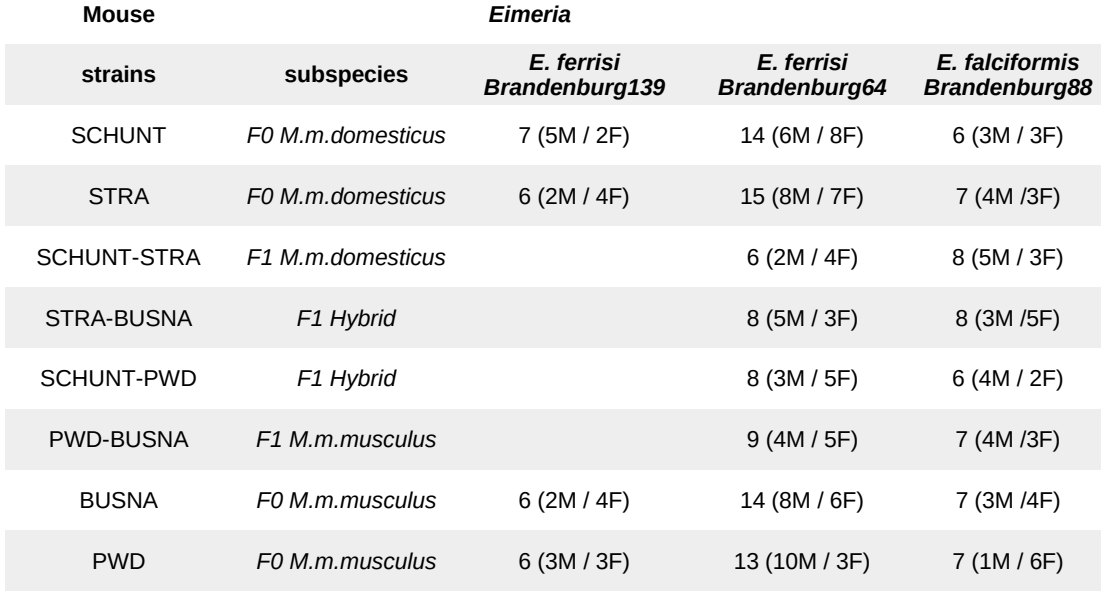
\includegraphics[width=6.92in,height=3.73in]{./media/image1.png}
	\end{FlushLeft}\end{figure}


%%%%%%%%%%%%%%%%%%%% Figure/Image No: 1 Ends here %%%%%%%%%%%%%%%%%%%%

\textbf{Table 1. Infection experiment design.}

 %%%%%%%%%%%%  Starting New Page here %%%%%%%%%%%%%%

\newpage
\par



%%%%%%%%%%%%%%%%%%%% Figure/Image No: 2 starts here %%%%%%%%%%%%%%%%%%%%

\begin{figure}[H]
	\begin{Center}
		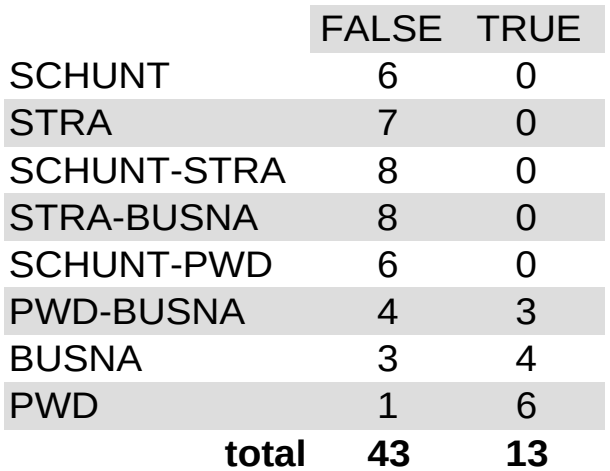
\includegraphics[width=2.26in,height=1.74in]{./media/image2.png}
	\end{Center}
\end{figure}


%%%%%%%%%%%%%%%%%%%% Figure/Image No: 2 Ends here %%%%%%%%%%%%%%%%%%%%

\par

{\fontsize{10pt}{12.0pt}\selectfont \textbf{\textcolor[HTML]{FF0000}{Table 2. Contingency table of mice infected with \textit{E. falciformis} isolate Brandenburg88 early death. }}\textcolor[HTML]{FF0000}{FALSE means that mice survived three days after oocysts shedding peak, TRUE that they died before. Chi-square test indicates that mouse strain influences the survival status (P<0.001). Only \textit{M. m. musculus} mice (PWD, BUSNA, or their F1) died early.}\par}

 %%%%%%%%%%%%  Starting New Page here %%%%%%%%%%%%%%

\newpage
\par

\begin{FlushLeft}
{\fontsize{14pt}{16.8pt}\selectfont \textbf{Figures}\par}
\end{FlushLeft}\par



%%%%%%%%%%%%%%%%%%%% Figure/Image No: 3 starts here %%%%%%%%%%%%%%%%%%%%

\begin{figure}[H]
	\begin{Center}
		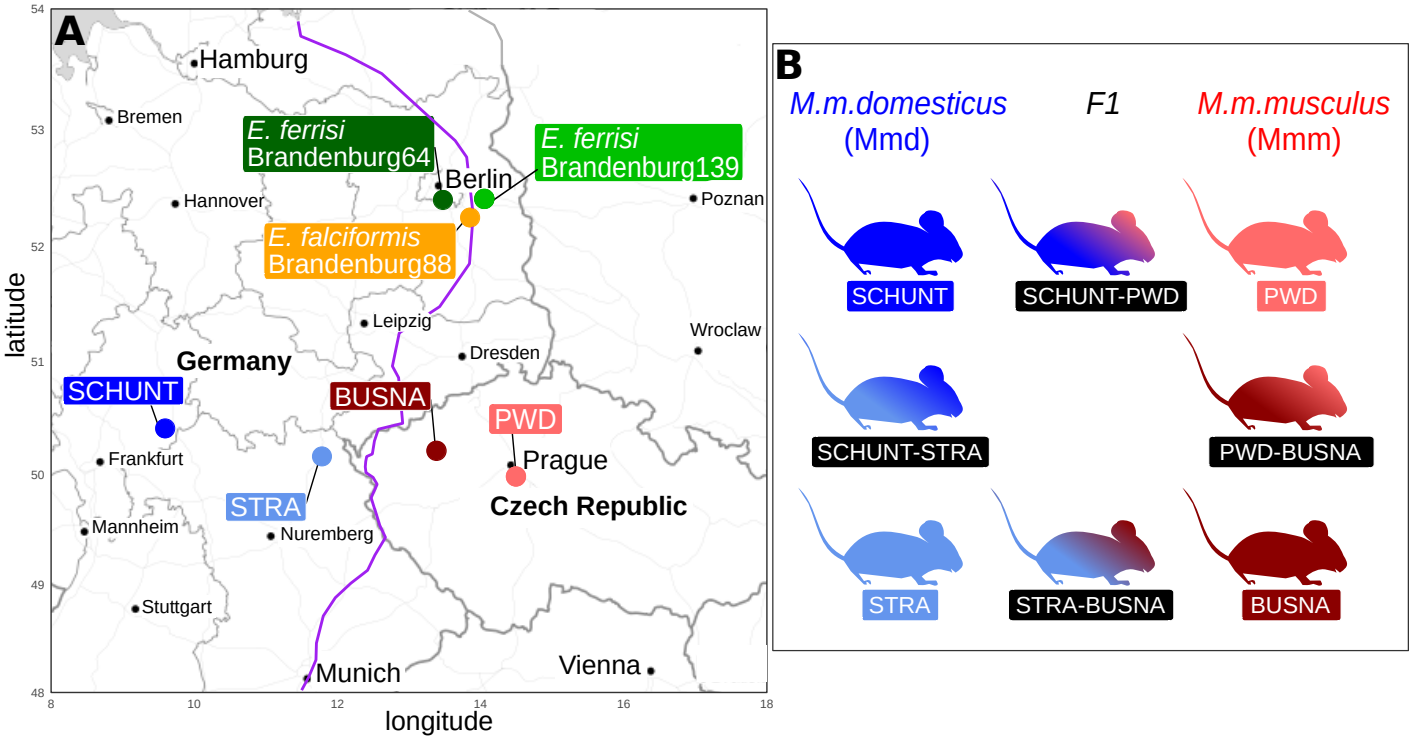
\includegraphics[width=6.92in,height=3.63in]{./media/image3.png}
	\end{Center}
\end{figure}


%%%%%%%%%%%%%%%%%%%% Figure/Image No: 3 Ends here %%%%%%%%%%%%%%%%%%%%

{\fontsize{10pt}{12.0pt}\selectfont \textbf{\textcolor[HTML]{CE181E}{Figure 1. Parasite isolates and mouse strains. }}(A)\textbf{ }Map showing locations at which mice were collected for breeding of mouse strains and isolation of parasites. The purple line is an estimation of the center of the house mouse hybrid zone between \textit{M. m. domesticus} and \textit{M. m. musculus} based on sampling and genotyping of mice in this area (Balard et al., 2020; Ďureje, Macholán, Baird, $\&$  Piálek, 2012, Macholán et al. 2019). \textcolor[HTML]{CE181E}{(B) The eight mouse strains (parents and F1s) used in our experimental infections.}\par}

 %%%%%%%%%%%%  Starting New Page here %%%%%%%%%%%%%%

\newpage
\par



%%%%%%%%%%%%%%%%%%%% Figure/Image No: 4 starts here %%%%%%%%%%%%%%%%%%%%

\begin{figure}[H]
	\begin{Center}
		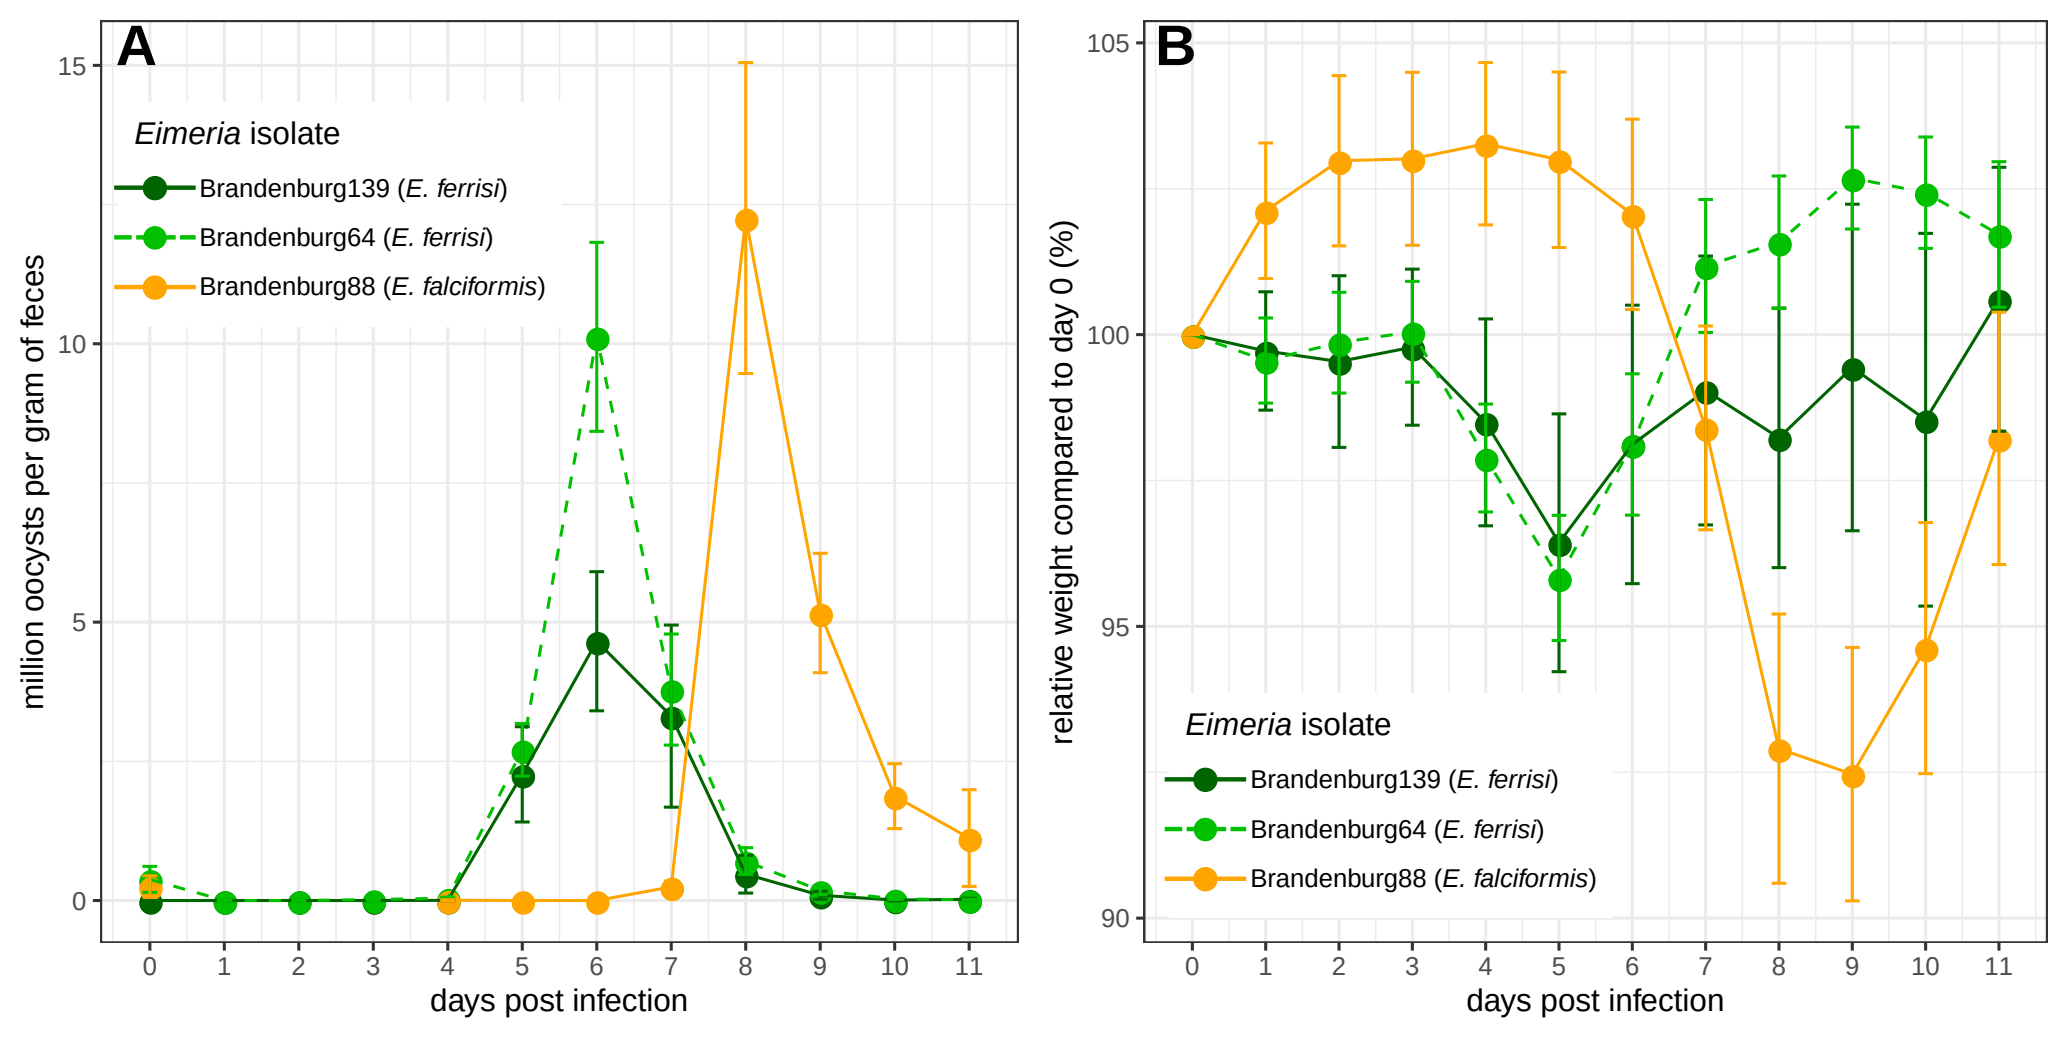
\includegraphics[width=7.52in,height=3.78in]{./media/image4.png}
	\end{Center}
\end{figure}


%%%%%%%%%%%%%%%%%%%% Figure/Image No: 4 Ends here %%%%%%%%%%%%%%%%%%%%

{\fontsize{10pt}{12.0pt}\selectfont \textbf{Figure 2. Parasite density (A) and relative weight (B) during \textit{Eimeria }infection. }Parasite density is calculated as number of oocysts detected (in millions) per gram of feces, relative weight is calculated as the percentage of weight compared to day 0.\textbf{ }Mean and 95$\%$  CI are plotted for each parasite isolate. All hosts strains are pooled together.\par}

 %%%%%%%%%%%%  Starting New Page here %%%%%%%%%%%%%%

\newpage
\par



%%%%%%%%%%%%%%%%%%%% Figure/Image No: 5 starts here %%%%%%%%%%%%%%%%%%%%

\begin{figure}[H]
	\begin{Center}
		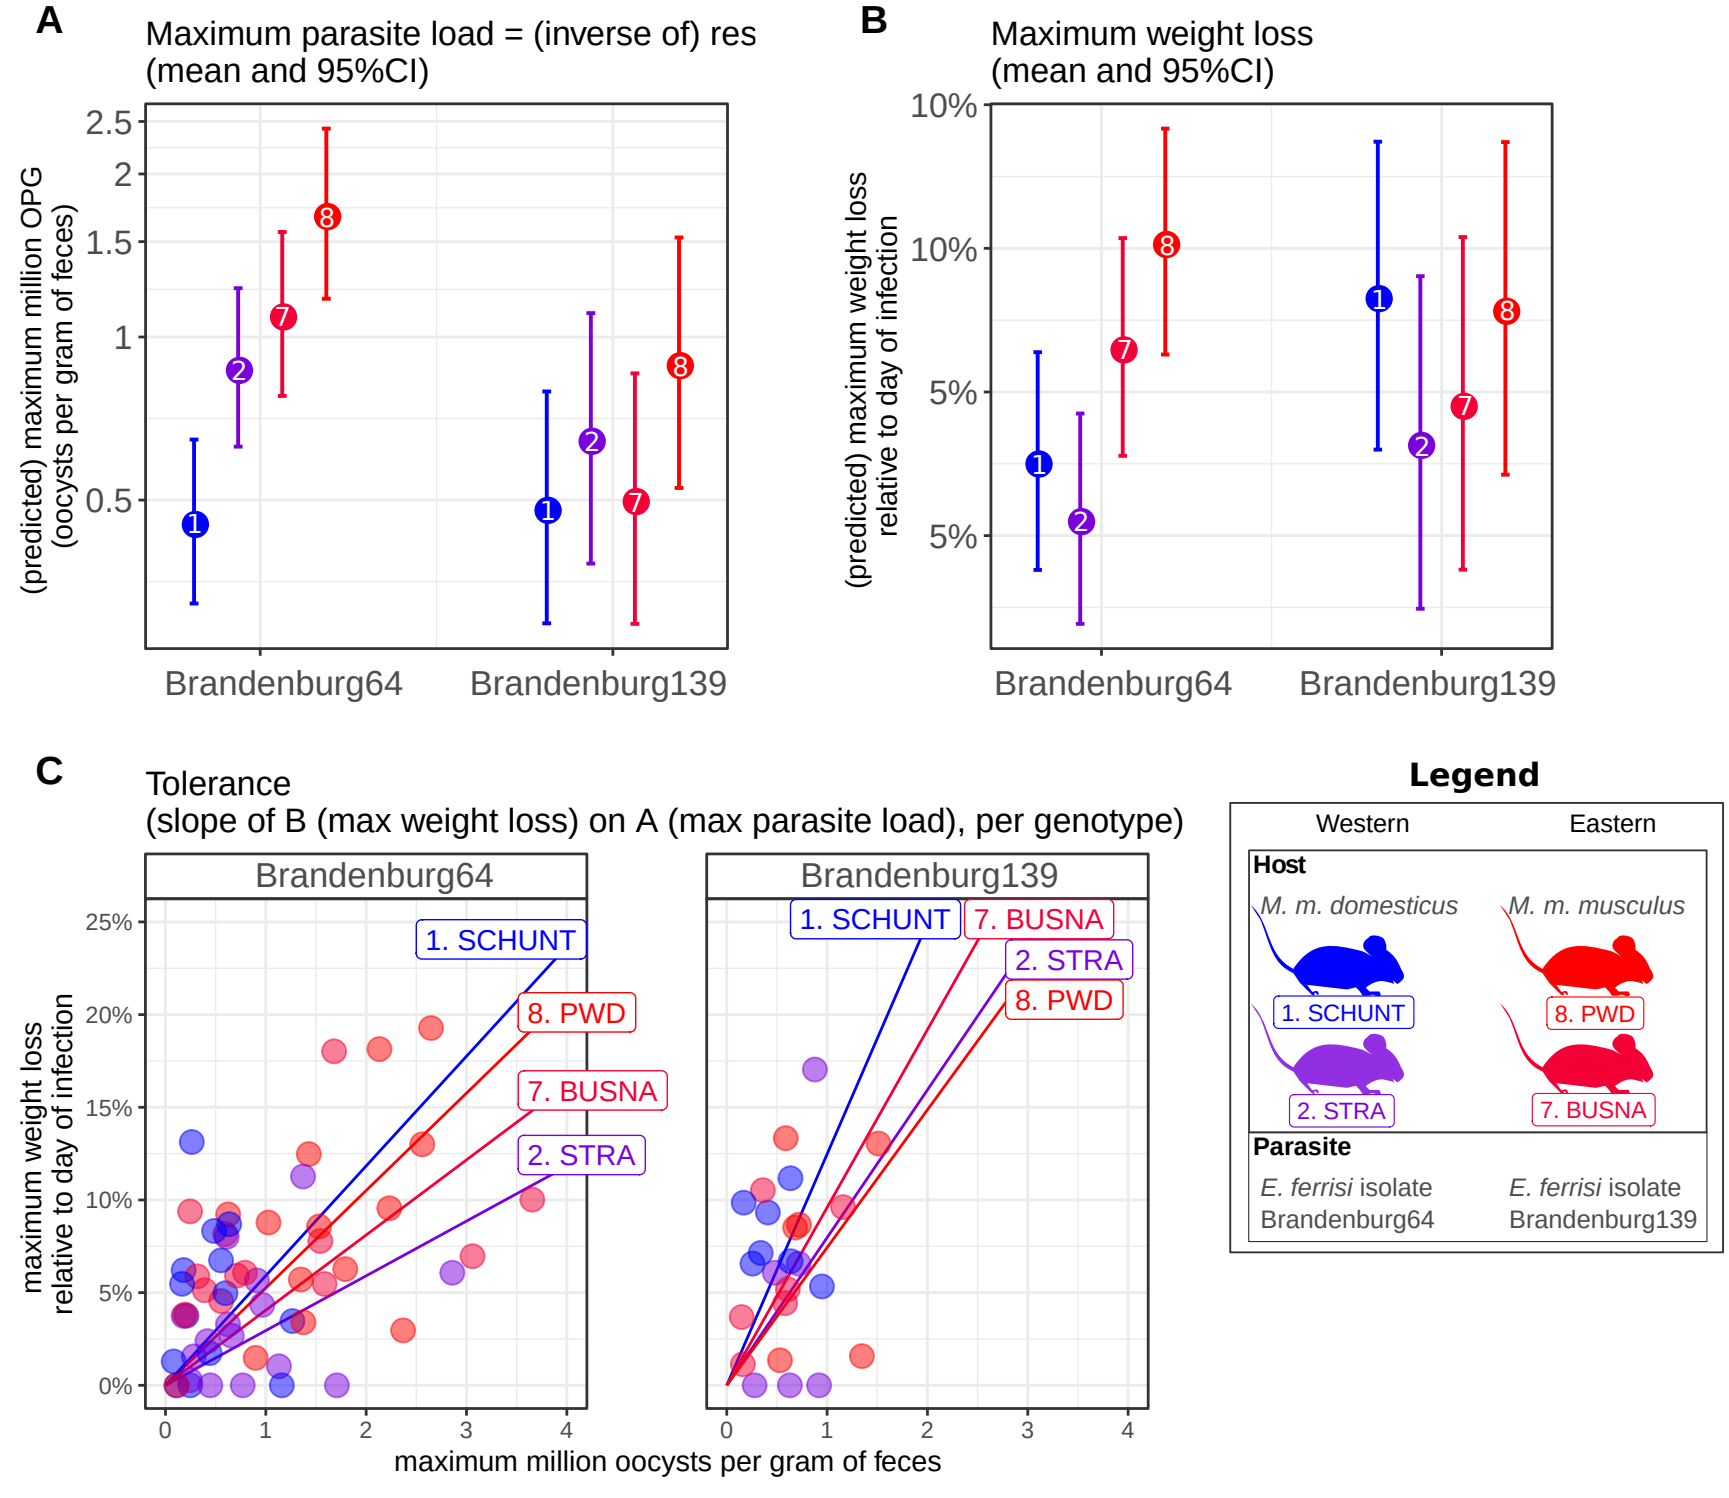
\includegraphics[width=5.63in,height=4.88in]{./media/image5.png}
	\end{Center}
\end{figure}


%%%%%%%%%%%%%%%%%%%% Figure/Image No: 5 Ends here %%%%%%%%%%%%%%%%%%%%

\par

{\fontsize{10pt}{12.0pt}\selectfont \textbf{Figure 3. Comparison of resistance, impact on weight and tolerance between mouse strain for both \textit{Eimeria ferrisi }isolates. }(A) Maximum oocysts per gram of feces used as a proxy for (inverse of) resistance; (B) Impact on host health measured as the maximum weight loss during patent period relative to starting weight ($\%$ ); (C) Tolerance estimated by the slope of the linear regression with null intercept modelling maximum relative weight loss as a response of maximum oocysts per gram of feces. A steep slope corresponds to a low tolerance.\par}\par

{\fontsize{10pt}{12.0pt}\selectfont \textcolor[HTML]{FF0000}{We did not detect (A) either higher parasite shedding of the Eastern parasite isolate in Eastern mouse strains and \textit{vice versa} or (C) higher tolerance of Eastern hosts infected by Eastern parasite isolate and \textit{vice versa}, thus our results do not support the hypothesis of local adaptation between \textit{E. ferrisi} and its host. }\par}

 %%%%%%%%%%%%  Starting New Page here %%%%%%%%%%%%%%

\newpage
\par



%%%%%%%%%%%%%%%%%%%% Figure/Image No: 6 starts here %%%%%%%%%%%%%%%%%%%%

\begin{figure}[H]
	\begin{Center}
		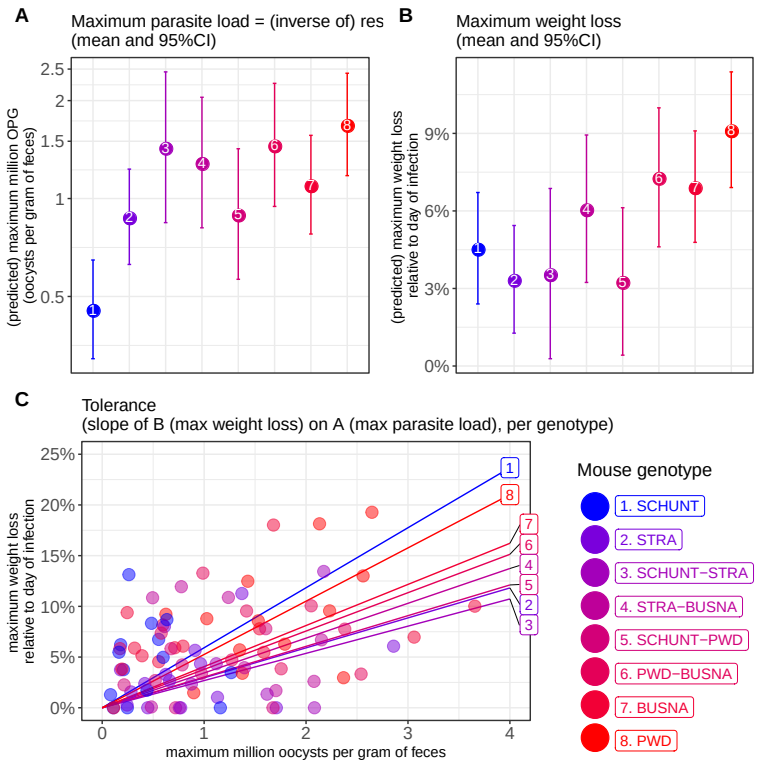
\includegraphics[width=5.53in,height=5.53in]{./media/image6.png}
	\end{Center}
\end{figure}


%%%%%%%%%%%%%%%%%%%% Figure/Image No: 6 Ends here %%%%%%%%%%%%%%%%%%%%

\par

{\fontsize{10pt}{12.0pt}\selectfont \textbf{Figure 4. Comparison of resistance, impact on weight and tolerance between mouse strain for \textit{E. ferrisi }isolate Brandenburg64. }(A) Maximum oocysts per gram of feces used as a proxy for (inverse of) resistance; (B) Impact on host health measured as the maximum weight loss during patent period relative to starting weight ($\%$ ); (C) Tolerance estimated by the slope of the linear regression with null intercept modelling maximum relative weight loss as a response of maximum oocysts per gram of feces. A steep slope corresponds to a low tolerance. \textcolor[HTML]{FF0000}{Maximum number of OPG and relative weight loss differ between mouse strains, but tolerance is similar.}\par}

 %%%%%%%%%%%%  Starting New Page here %%%%%%%%%%%%%%

\newpage
\par



%%%%%%%%%%%%%%%%%%%% Figure/Image No: 7 starts here %%%%%%%%%%%%%%%%%%%%

\begin{figure}[H]
	\begin{Center}
		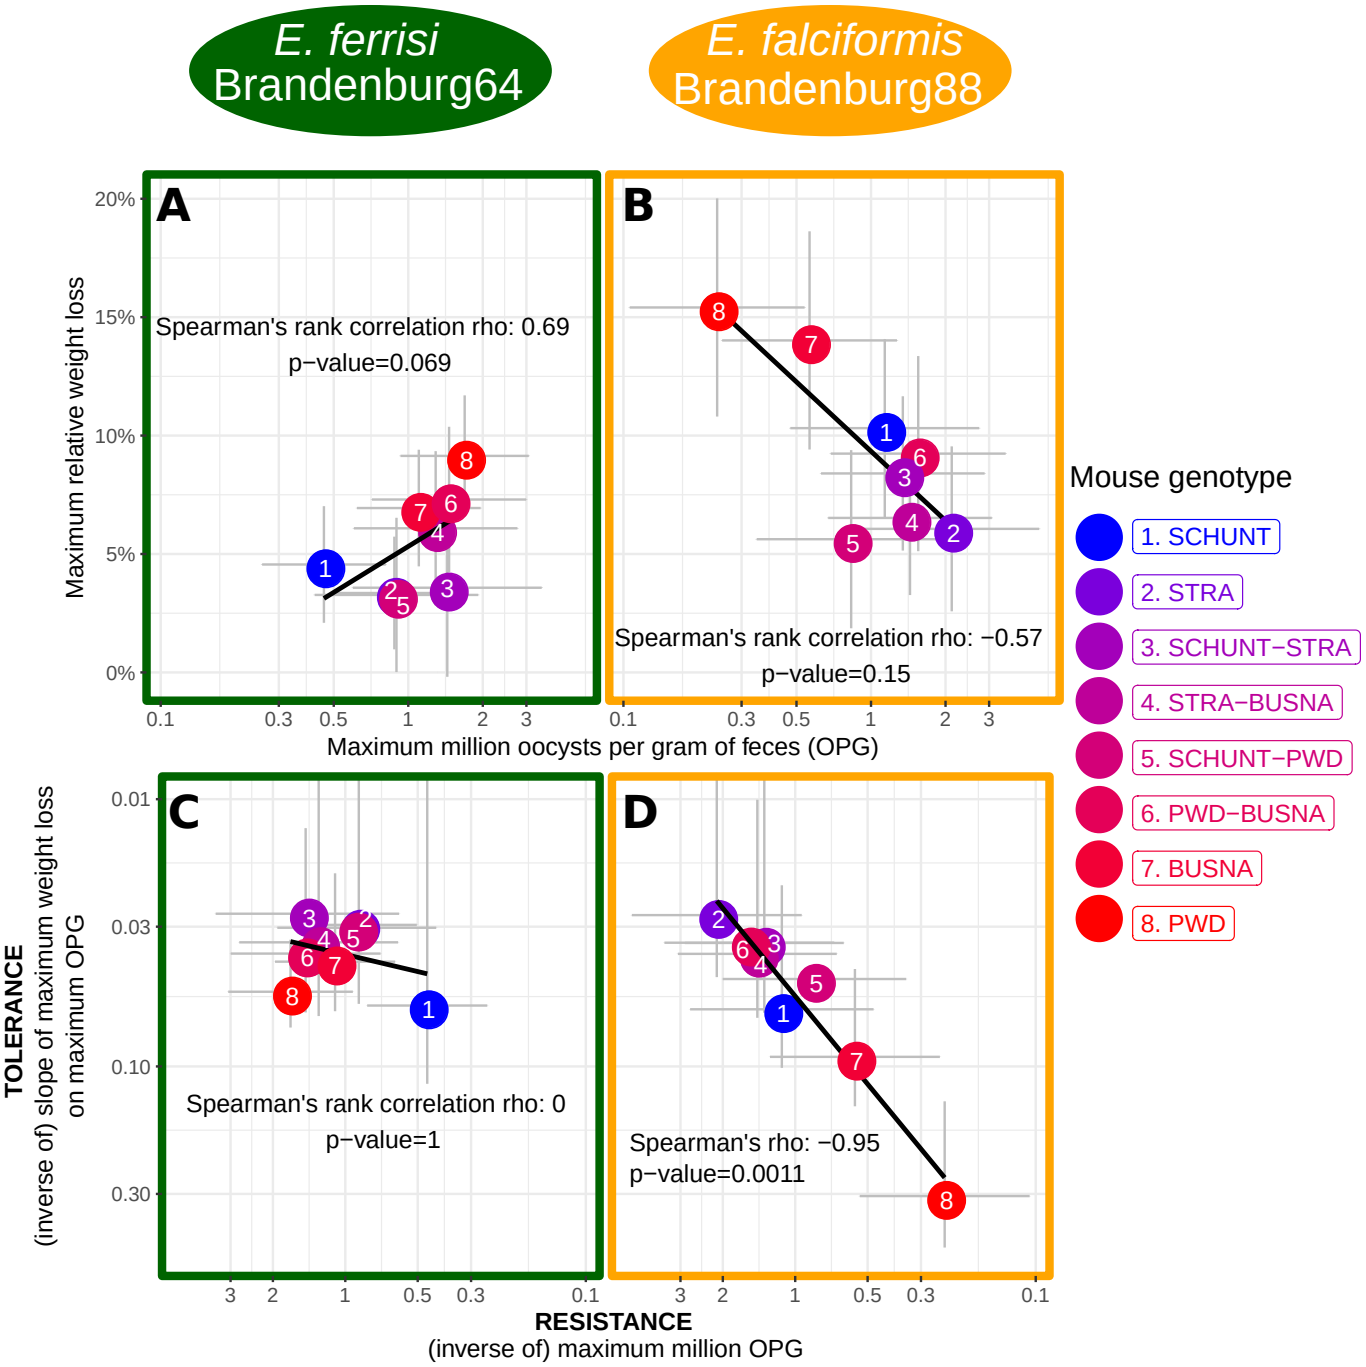
\includegraphics[width=5.8in,height=5.81in]{./media/image7.png}
	\end{Center}
\end{figure}


%%%%%%%%%%%%%%%%%%%% Figure/Image No: 7 Ends here %%%%%%%%%%%%%%%%%%%%

\par

{\fontsize{10pt}{12.0pt}\selectfont \textbf{\textcolor[HTML]{FF0000}{Figure 5. Resistance-tolerance coupling.}}\textcolor[HTML]{FF0000}{ Correlation between mean parasite load and mean relative weight loss (A, B) and between resistance and tolerance (C, D) for both \textit{Eimeria} species. (A,B): maximum relative weight loss on maximum oocysts per gram of feces; (C, D):\textbf{ }tolerance (slope of the linear regression with null intercept modelling maximum relative weight loss as a response of maximum oocysts per gram of feces, a high value corresponding to a low tolerance) on resistance (maximum oocysts per gram of feces used as a proxy, a high value corresponding to a low resistance); Grey error bars represent 95$\%$  confidence intervals. No indication of coupling between resistance and tolerance \textit{E. ferrisi }isolate Brandenburg64, negative correlation between resistance and tolerance for \textit{E. falciformis }isolate Brandenburg88. }\par}

 %%%%%%%%%%%%  Starting New Page here %%%%%%%%%%%%%%

\newpage
\par


\vspace{\baselineskip}


%%%%%%%%%%%%%%%%%%%% Figure/Image No: 8 starts here %%%%%%%%%%%%%%%%%%%%

\begin{figure}[H]
	\begin{Center}
		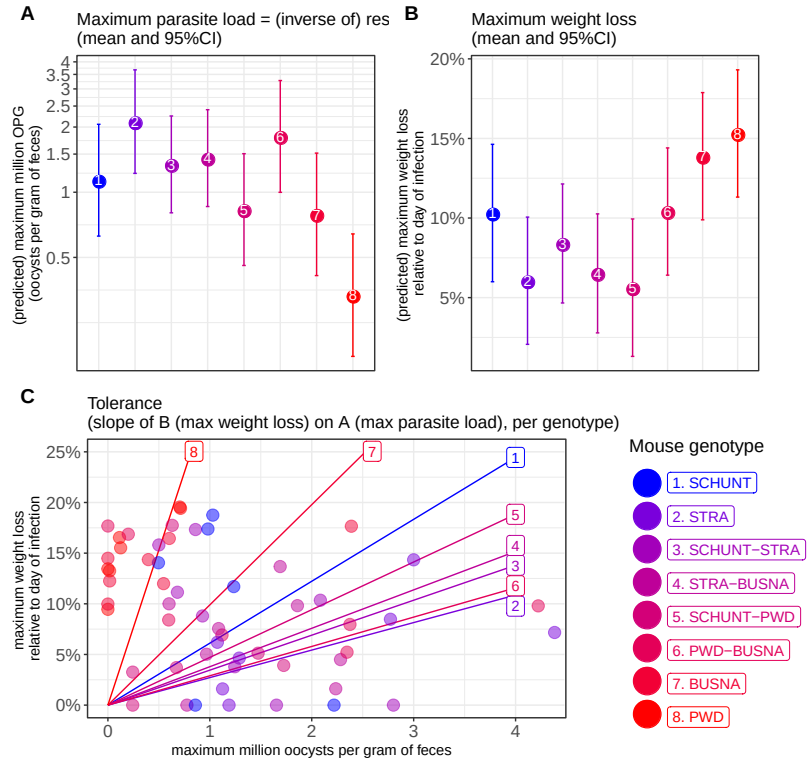
\includegraphics[width=5.74in,height=5.46in]{./media/image8.png}
	\end{Center}
\end{figure}


%%%%%%%%%%%%%%%%%%%% Figure/Image No: 8 Ends here %%%%%%%%%%%%%%%%%%%%

\par

{\fontsize{10pt}{12.0pt}\selectfont \textbf{Figure 6. Comparison of resistance, impact on weight and tolerance between mouse strain for \textit{E. ferrisi }isolate Brandenburg88. }(A) Maximum oocysts per gram of feces used as a proxy for (inverse of) resistance; (B) Impact on host health measured as the maximum weight loss during patent period relative to starting weight ($\%$ ); (C) Tolerance estimated by the slope of the linear regression with null intercept modelling maximum relative weight loss as a response of maximum oocysts per gram of feces. A steep slope corresponds to a low tolerance. \textcolor[HTML]{FF0000}{Maximum number of OPG, relative weight loss and tolerance differ between mouse strains.}\par}

 %%%%%%%%%%%%  Starting New Page here %%%%%%%%%%%%%%

\newpage
\par

\begin{FlushLeft}
{\fontsize{14pt}{16.8pt}\selectfont \textbf{Supplementary material}\par}
\end{FlushLeft}\par



%%%%%%%%%%%%%%%%%%%% Figure/Image No: 9 starts here %%%%%%%%%%%%%%%%%%%%

\begin{figure}[H]
	\begin{Center}
		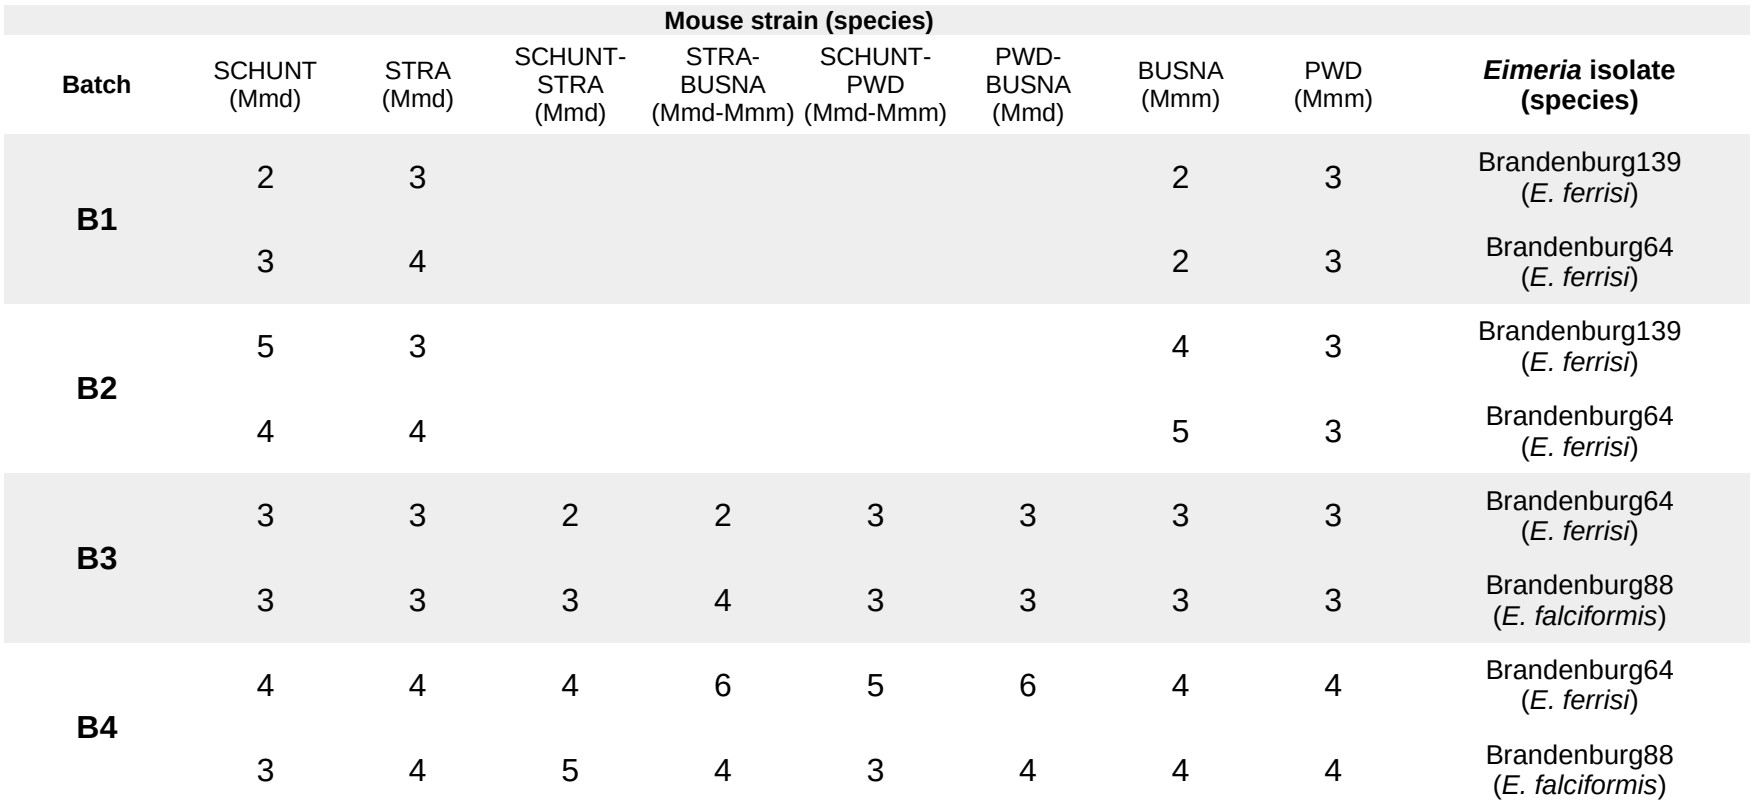
\includegraphics[width=6.92in,height=3.18in]{./media/image9.png}
	\end{Center}
\end{figure}


%%%%%%%%%%%%%%%%%%%% Figure/Image No: 9 Ends here %%%%%%%%%%%%%%%%%%%%

\textbf{Supplementary Table S1. Chronology of experimental \textcolor[HTML]{CE181E}{infections}}

 %%%%%%%%%%%%  Starting New Page here %%%%%%%%%%%%%%

\newpage
\par

\begin{FlushLeft}
{\fontsize{14pt}{16.8pt}\selectfont \textbf{Funding }\par}
\end{FlushLeft}\par

This work was funded by the German Research Foundation (DFG) Grant [HE 7320/1-1] to EH. VHJ is an associated student of GRK 2046 funded by the DFG. The maintenance of wild-derived strains was supported by the ROSE program from Czech Academy of Sciences and the Czech Science Foundation (project 16-23773S) to JP.\par

{\fontsize{14pt}{16.8pt}\selectfont \textbf{References}\par}\par

\begin{FlushLeft}
Al-khlifeh, E., Balard, A., Jarquín-Díaz, V. H., Weyrich, A., Wibbelt, G., $\&$  Heitlinger, E. (2019). \textit{Eimeria falciformis BayerHaberkorn1970 and novel wild derived isolates from house mice: Differences in parasite lifecycle, pathogenicity and host immune reactions. BioRxiv. doi: 10.1101/611277}
\end{FlushLeft}\par

\begin{FlushLeft}
Anderson, R. M., $\&$  May, R. M. (1982). Coevolution of hosts and parasites. \textit{Parasitology, 85 (Pt 2), 411–426. doi: 10.1017/s0031182000055360}
\end{FlushLeft}\par

\begin{FlushLeft}
Ankrom, S. L., Chobotar, B., $\&$  Ernst, J. V. (1975). Life cycle of \textit{Eimeria ferrisi Levine $\&$  Ivens, 1965 in the Mouse, Mus musculus. The Journal of Protozoology, 22(3), 317–323. doi: 10.1111/j.1550-7408.1975.tb05177.x}
\end{FlushLeft}\par

\begin{FlushLeft}
Ayres, J. S., $\&$  Schneider, D. S. (2012). Tolerance of Infections. \textit{Annual Review of Immunology}, 30(1), 271–294. doi: 10.1146/annurev-immunol-020711-075030
\end{FlushLeft}\par

\begin{FlushLeft}
Baird, S. J. E., $\&$  Goüy de Bellocq, J. (2019). Shifting paradigms for studying parasitism in hybridising hosts: Response to Theodosopoulos, Hund, and Taylor. \textit{Trends in Ecology $\&$  Evolution, 34, 387–389. doi: 10.1016/j.tree.2019.01.011}
\end{FlushLeft}\par

\begin{FlushLeft}
Baird, S. J. E., Ribas, A., Macholán, M., Albrecht, T., Piálek, J., $\&$  Goüy de Bellocq, J. (2012). Where are the wormy mice? A reexamination of hybrid parasitism in the European house mouse hybrid zone. \textit{Evolution, 66(9), 2757–2772. doi: 10.1111/j.1558-5646.2012.01633.x}
\end{FlushLeft}\par

\begin{FlushLeft}
Balard, A., Jarquín‐Díaz, V. H., Jost, J., Martincová, I., Ďureje, Ľ., Piálek, J., Macholán, M., Goüy de Bellocq, J., Baird, S. J. E., $\&$  Heitlinger, E. (2020). Intensity of infection with intracellular Eimeria spp. and pinworms is reduced in hybrid mice compared to parental subspecies. \textit{Journal of Evolutionary Biology}, 33(4), 435–448. doi: 10.1111/jeb.13578
\end{FlushLeft}\par

\begin{FlushLeft}
\textcolor[HTML]{1C1D1E}{Baucom, R. S., $\&$  de Roode, J. C. (2011). Ecological immunology and tolerance in plants and animals. \textit{Functional Ecolog}}\textit{y}, 25(1), 18–28. doi: 10.1111/j.1365-2435.2010.01742.x
\end{FlushLeft}\par

\begin{FlushLeft}
Boots, M., Best, A., Miller, M. R., $\&$  White, A. (2008). The role of ecological feedbacks in the evolution of host defence: what does theory tell us? Philosophical Transactions of the Royal Society B: Biological Sciences, 364(1513), 27–36. doi: 10.1098/rstb.2008.0160
\end{FlushLeft}\par

\begin{FlushLeft}
\textcolor[HTML]{FF0000}{Brett, M. T., 2004. When is a correlation between non-independent variables $``$spurious$"$ ? Oikos 105, 647–656. doi: 10.1111/j.0030-1299.2004.12777.x}
\end{FlushLeft}\par

\begin{FlushLeft}
Carval, D., $\&$  Ferriere, R. (2010). A unified model for the coevolution of resistance, tolerance, and virulence. Evolution, 64(10):2988-3009. doi: 10.1111/j.1558-5646.2010.01035.x
\end{FlushLeft}\par

\begin{FlushLeft}
Chapman, H. D., Barta, J. R., Blake, D., Gruber, A., Jenkins, M., Smith, N. C., $ \ldots $  Tomley, F. M. (2013). A selective review of advances in coccidiosis research. Advances in Parasitology, 83, 93–171. doi: 10.1016/B978-0-12-407705-8.00002-1
\end{FlushLeft}\par

\begin{FlushLeft}
Clerc, M., Fenton, A., Babayan, S. A., $\&$  Pedersen, A. B. (2019). Parasitic nematodes simultaneously suppress and benefit from coccidian coinfection in their natural mouse host. \textit{Parasitology, 146(8), 1096–1106. doi: 10.1017/S0031182019000192}
\end{FlushLeft}\par

\begin{FlushLeft}
Delignette-Muller, M. L., $\&$  Dutang, C. (2015). fitdistrplus: An R Package for Fitting Distributions. \textit{Journal of Statistical Software, 64(4), 1–34.}
\end{FlushLeft}\par

\begin{FlushLeft}
Ďureje, Ľ., Macholán, M., Baird, S. J., $\&$  Piálek, J. (2012). The mouse hybrid zone in Central Europe: From morphology to molecules. \textit{Folia Zoologica, 61(3–4), 308–318.}
\end{FlushLeft}\par

\begin{FlushLeft}
Ehret, T., Spork, S., Dieterich, C., Lucius, R., $\&$  Heitlinger, E. (2017). Dual RNA-seq reveals no plastic transcriptional response of the coccidian parasite \textit{Eimeria falciformis to host immune defenses. BMC Genomics, 18(1), 686. doi: 10.1186/s12864-017-4095-6}
\end{FlushLeft}\par

\begin{FlushLeft}
Floyd, R. M., Rogers, A. D., Lambshead, P. J. D., $\&$  Smith, C. R. (2005). Nematode-specific PCR primers for the 18S small subunit rRNA gene. \textit{Molecular Ecology Notes}, \textit{5}(3), 611–612. doi: 10.1111/j.1471-8286.2005.01009.x
\end{FlushLeft}\par

\begin{FlushLeft}
\textcolor[HTML]{FF0000}{Gandon, S., $\&$  Michalakis, Y. (2000). Evolution of parasite virulence against qualitative or quantitative host resistance. \textit{Proceedings of the Royal Society B: Biological Sciences}, 267(1447), 985–990. doi: 10.1098/rspb.2000.1100}
\end{FlushLeft}\par

\begin{FlushLeft}
Graham, A. L., Allen, J. E., $\&$  Read, A. F. (2005). Evolutionary causes and consequences of immunopathology. \textit{Annual Review of Ecology, Evolution, and Systematics, 373–397. doi: 10.1146/annurev.ecolsys.36.102003.152622}
\end{FlushLeft}\par

\begin{FlushLeft}
Gregorová, S., $\&$  Forejt, J. (2000). PWD/Ph and PWK/Ph inbred mouse strains of \textit{Mus m. Musculus subspecies-a valuable resource of phenotypic variations and genomic polymorphisms. Folia Biologica, 46(1), 31–41.}
\end{FlushLeft}\par

\textcolor[HTML]{FF0000}{Guivier, E., Galan, M., Salvador, A. R., Xuéreb, A., Chaval, Y., Olsson, G. E., $ \ldots $  Charbonnel, N. (2010). Tnf-$ \alpha $  expression and promoter sequences reflect the balance of tolerance/resistance to Puumala hantavirus infection in European bank vole populations. Infection, Genetics and Evolution, 10(8), 1208–1217. doi: 10.1016/j.meegid.2010.07.022}\par

\begin{FlushLeft}
Haberkorn, A. (1970). Die Entwicklung von \textit{Eimeria falciformis (Eimer 1870) in der weißen Maus (Mus musculus). Zeitschrift für Parasitenkunde, 34(1), 49–67. doi: 10.1007/BF00629179}
\end{FlushLeft}\par

\begin{FlushLeft}
Howick, V. M., $\&$  Lazzaro, B. P. (2017). The genetic architecture of defence as resistance to and tolerance of bacterial infection in \textit{Drosophila melanogaster}. \textit{Molecular Ecology}, \textit{26}(6), 1533–1546. doi: 10.1111/mec.14017 
\end{FlushLeft}\par

\begin{FlushLeft}
Jackman, S. (2017). pscl: classes and methods for R developed in the political science computational laboratory. United States Studies Centre, University of Sydney. R package version 1.5.2. \href{https://github.com/atahk/pscl/}{https://github.com/atahk/pscl/}
\end{FlushLeft}\par

\begin{FlushLeft}
Janzen, D. H. (1980). When is it coevolution? \textit{Evolution}, 34(3), 611–612. doi: 10.1111/j.1558-5646.1980.tb04849.x
\end{FlushLeft}\par

\begin{FlushLeft}
Jarquín-Díaz, V. H., Balard, A., Jost, J., Kraft, J., Dikmen, M. N., Kvičerová, J., $\&$  Heitlinger, E. (2019). Detection and quantification of house mouse \textit{Eimeria at the species level – Challenges and solutions for the assessment of coccidia in wildlife. International Journal for Parasitology: Parasites and Wildlife, 10, 29–40. doi: 10.1016/j.ijppaw.2019.07.004}
\end{FlushLeft}\par

\begin{FlushLeft}
Kaltz, O., $\&$  Shykoff, J. Local adaptation in host–parasite systems. \textit{Heredity} \textbf{81, }361–370 (1998). doi: 10.1046/j.1365-2540.1998.00435.x
\end{FlushLeft}\par

\begin{FlushLeft}
Klemme, I., $\&$  Karvonen, A. (2016). Vertebrate defense against parasites: Interactions between avoidance, resistance, and tolerance. \textit{Ecology and Evolution}, \textit{7}(2), 561–571. doi: 10.1002/ece3.2645
\end{FlushLeft}\par

\begin{FlushLeft}
\href{https://www.zotero.org/google-docs/?I2LRxy}{Kutzer, M. A. M., $\&$  Armitage, S. A. O. (2016). Maximising fitness in the face of parasites: A review of host tolerance. }\href{https://www.zotero.org/google-docs/?I2LRxy}{\textit{Zoology}\href{https://www.zotero.org/google-docs/?I2LRxy}{}, }\href{https://www.zotero.org/google-docs/?I2LRxy}{\textit{119}}(4), 281–289. doi: 10.1016/j.zool.2016.05.011
\end{FlushLeft}\par

\begin{FlushLeft}
Lefèvre, T., Williams, A. J., $\&$  de Roode, J. C. (2010). Genetic variation in resistance, but not tolerance, to a protozoan parasite in the monarch butterfly. \textit{Proceedings of the Royal Society B: Biological Sciences}, 278(1706), 751–759. doi: 10.1098/rspb.2010.1479
\end{FlushLeft}\par

\begin{FlushLeft}
Little, T. J., Shuker, D. M., Colegrave, N., Day, T., $\&$  Graham, A. L. (2010). The coevolution of virulence: Tolerance in perspective. \textit{PLOS Pathogens, 6(9), e1001006. doi: 10.1371/journal.ppat.1001006}
\end{FlushLeft}\par

\begin{FlushLeft}
Lüdecke D (2018). ggeffects: tidy data frames of marginal effects from regression models. Journal of Open Source Software, 3(26), 772. doi: 10.21105/joss.00772
\end{FlushLeft}\par

\textcolor[HTML]{00000A}{Macholán M., Baird S.J.E., Fornuskova A., Martincová I., Rubík, P., Ďureje Ľ., Heitlinger E., Piálek J. 2019. Widespread introgression of the \textit{Mus musculus musculus Y chromosome in Central Europe. BioRxiv. doi:\href{http://dx.doi.org/10.1101/2019.12.23.887471}{ }\href{http://dx.doi.org/10.1101/2019.12.23.887471}{10.1101/2019.12.23.887471}}}\par

\begin{FlushLeft}
Martincová, I., Ďureje, Ľ., Kreisinger, J., Macholán, M., $\&$  Piálek, J. (2019). Phenotypic effects of the Y chromosome are variable and structured in hybrids among house mouse recombinant lines. \textit{Ecology and Evolution, 9(10), 6124–6137. doi: 10.1002/ece3.5196}
\end{FlushLeft}\par

\begin{FlushLeft}
Mazé-Guilmo, E., Loot, G., Páez, D. J., Lefèvre, T., $\&$  Blanchet, S. (2014). Heritable variation in host tolerance and resistance inferred from a wild host–parasite system. \textit{Proceedings of the Royal Society B: Biological Sciences}, 281(1779), 20132567. doi: 10.1098/rspb.2013.2567
\end{FlushLeft}\par

\begin{FlushLeft}
Medzhitov, R., Schneider, D. S., $\&$  Soares, M. P. (2012). Disease tolerance as a defense strategy. \textit{Science}, \textit{335}(6071), 936–941. doi: 10.1126/science.1214935
\end{FlushLeft}\par

\begin{FlushLeft}
Piálek, J., Vyskocilová, M., Bímová, B., Havelková, D., Piálková, J., Dufková, P., Bencová, V., Dureje, L., Albrecht, T., Hauffe, H. C., Macholán, M., Munclinger, P., Storchová, R., Zajícová, A., Holán, V., Gregorová, S., $\&$  Forejt, J. (2008). Development of unique house mouse resources suitable for evolutionary studies of speciation. \textit{The Journal of Heredity, 99(1), 34–44. doi: 10.1093/jhered/esm083}
\end{FlushLeft}\par

\begin{FlushLeft}
R Development Core Team. (2018). \textit{R: A language and environment for statistical computing. R Foundation for Statistical Computing, Vienna, Austria. http://www.R-project.org}
\end{FlushLeft}\par

\begin{FlushLeft}
Råberg, L., Sim, D., $\&$  Read, A. F. (2007). Disentangling genetic variation for resistance and tolerance to infectious diseases in animals. \textit{Science, 318(5851), 812–814. doi: 10.1126/science.1148526}
\end{FlushLeft}\par

\begin{FlushLeft}
Råberg, L., Graham, A. L., $\&$  Read, A. F. (2009). Decomposing health: Tolerance and resistance to parasites in animals. \textit{Philosophical Transactions of the Royal Society B: Biological Sciences, 364(1513), 37–49. doi: 10.1098/rstb.2008.0184}
\end{FlushLeft}\par

\begin{FlushLeft}
Restif, O., $\&$  Koella, J. C. (2004). Concurrent evolution of resistance and tolerance to pathogens. \textit{The American Naturalist}, \textit{164}(4). doi: 10.1086/423713
\end{FlushLeft}\par

\begin{FlushLeft}
Rose, M. E., Hesketh, P., $\&$  Wakelin, D. (1992). Immune control of murine coccidiosis: CD4+ and CD8+ T lymphocytes contribute differentially in resistance to primary and secondary infections. \textit{Parasitology, 105, 349–354. doi: 10.1017/s0031182000074515}
\end{FlushLeft}\par

\begin{FlushLeft}
Roy, B. A., $\&$  Kirchner, J. W. (2000). Evolutionary dynamics of pathogen resistance and tolerance. \textit{Evolution, 54(1), 51–63. doi: 10.1111/j.0014-3820.2000.tb00007.x}
\end{FlushLeft}\par

\begin{FlushLeft}
Schito,\textcolor[HTML]{00000A}{ M. L., Barta, J. R., $\&$  Chobotar, B. (1996). Comparison of four murine \textit{Eimeria} species in immunocompetent and immunodeficient mice. \textit{The Journal of Parasitology}, \textit{82}(2), 255–262. doi: 10.2307/3284157}
\end{FlushLeft}\par

\begin{FlushLeft}
\textcolor[HTML]{00000A}{Shaw, D. J., $\&$  Dobson, A. P. (1995). Patterns of macroparasite abundance and aggregation in wildlife populations: A quantitative review.\textit{Parasitology}, \textbf{11}(S1), S111–S127. \href{https://doi.org/10.1017/S0031182000075855}{doi: 10.1017S0031182000075855}}
\end{FlushLeft}\par

\begin{FlushLeft}
Sheldon, B. C., $\&$  Verhulst, S. (1996). Ecological immunology: Costly parasite defences and trade-offs in evolutionary ecology. \textit{\textcolor[HTML]{00000A}{Trends in Ecology $\&$  Evolution, 11(8), 317–321. doi: 10.1016/0169-5347(96)10039-2 }}
\end{FlushLeft}\par

\begin{FlushLeft}
Schmid-Hempel, P. (2013). Evolutionary parasitology: the integrated study of infections, immunology, ecology, and genetics. Oxford University Press. doi:10.1093/acprof:oso/9780199229482.001.0001
\end{FlushLeft}\par

\begin{FlushLeft}
\textcolor[HTML]{1C1D1E}{Simms, E.L. (2000) Defining tolerance as a norm of reaction. \textit{Evolutionary Ecology}, 14, 563–570. doi: 10.1023/A:1010956716539}
\end{FlushLeft}\par

\begin{FlushLeft}
Smith, A. L., $\&$  Hayday, A. C. (2000). Genetic dissection of primary and secondary responses to a widespread natural pathogen of the gut, \textit{Eimeria vermiformis. Infection and Immunity, 68(11), 6273–6280. doi: 10.1128/iai.68.11.6273-6280.2000}
\end{FlushLeft}\par

\begin{FlushLeft}
Soares, M. P., Teixeira, L., $\&$  Moita, L. F. (2017). Disease tolerance and immunity in host protection against infection. \textit{Nature Reviews Immunology, 17(2), 83–96. doi: 10.1038/nri.2016.136}
\end{FlushLeft}\par

\begin{FlushLeft}
Stange, J., Hepworth, M. R., Rausch, S., Zajic, L., Kühl, A. A., Uyttenhove, C., Renauld, J.-C., Hartmann, S., $\&$  Lucius, R. (2012). IL-22 mediates host defense against an intestinal intracellular parasite in the absence of IFN-$ \gamma $  at the cost of Th17-driven immunopathology. \textit{Journal of Immunology, 188(5), 2410–2418. doi: 10.4049/jimmunol.1102062 }
\end{FlushLeft}\par

\begin{FlushLeft}
Vale, P. F., $\&$  Little, T. J. (2012). Fecundity compensation and tolerance to a sterilizing pathogen in Daphnia. \textit{Journal of Evolutionary Biology,} 25(9), 1888–1896. doi: 10.1111/j.1420-9101.2012.02579.x
\end{FlushLeft}\par

\begin{FlushLeft}
Venables, W. N., $\&$  Ripley, B. D. (2002). Modern Applied Statistics with S (Fourth edition). New York, NY: Springer.
\end{FlushLeft}\par

\begin{FlushLeft}
Wickham, H. (2016). Ggplot2: Elegant graphics for data analysis (Second edition). New York, NY: Springer.
\end{FlushLeft}\par

\begin{FlushLeft}
Woolhouse, M., Webster, J., Domingo, E., Charlesworth, B., $\&$  Levin, B.R. (2002) Biological and biomedical implications of the co-evolution of pathogens and their hosts. \textit{Nature Genetics}, 32, 569–577 (2002). doi: \href{https://doi.org/10.1038/ng1202-569}{10.1038/ng1202-569}
\end{FlushLeft}\par

\begin{FlushLeft}
Zeileis, A., Kleiber, C., $\&$  Jackman, S. (2008). Regression models for count data in R. Journal of Statistical Software 27(8). doi: 10.18637/JSS.V027.I08 
\end{FlushLeft}\par


\printbibliography
\end{document}